\documentclass[sigconf,review,anonymous]{acmart}

\usepackage{amsmath,amsfonts}
\usepackage{algorithmic}
\usepackage{graphicx}
\usepackage{textcomp}
\usepackage{xcolor}
\usepackage{ifthen}
\usepackage{balance}

% cleveref
\usepackage{hyperref}
\usepackage[nameinlink]{cleveref}
\crefname{section}{\S}{Sections}
\crefname{figure}{Fig.}{Figs.}
\Crefname{figure}{Figure}{Figures}
\crefname{table}{Table}{Tables}

% tikz
\usepackage{tikz,pgfplots}
\usetikzlibrary{positioning}

% for subfigures
\usepackage[caption=false,font=footnotesize]{subfig}

% for scientific notation like 1e-8
\usepackage{siunitx}
\sisetup{output-exponent-marker=\ensuremath{\mathrm{e}}}

\newcommand{\dims}[1]{\langle #1 \rangle}

% macros for plots
\newcommand{\datafile}{}
\newcommand{\threads}{}
\newcommand{\set}{}

\newcommand{\GB}[1]{\textcolor{red}{\textbf{GB}: #1}}
\newcommand{\JW}[1]{\textcolor{blue}{\textbf{JW}: #1}}
\newcommand{\RZ}[1]{\textcolor{purple}{\textbf{RZ}: #1}}


\acmConference[ICPP'21]{International Conference on Parallel Processing}{August 9--12}{Chicago, IL, USA}


\title{Accelerating Neural Network Training using Arbitrary Precision Approximating Matrix Multiplication Algorithms
%\thanks{Identify applicable funding agency here. If none, delete this.}
}

\author{\IEEEauthorblockN{Grey Ballard}
\IEEEauthorblockA{\textit{Department of Computer Science} \\
\textit{Wake Forest University}\\
Winston-Salem, NC, USA \\
\email{ballard@wfu.edu}}
\and
\IEEEauthorblockN{Jack Weissenberger}
\IEEEauthorblockA{\textit{Department of Computer Science} \\
\textit{Wake Forest University}\\
Winston-Salem, NC, USA \\
\email{jack.weissenberger@gmail.com}}
\and
\IEEEauthorblockN{Luoping Zhang}
\IEEEauthorblockA{\textit{Department of Computer Science} \\
\textit{Wake Forest University}\\
Winston-Salem, NC, USA \\
\email{zhanl317@wfu.edu}}
}

\begin{abstract}
Matrix multiplication is one of the bottleneck computations for training the weights within deep neural networks.
To speed up the training phase, we propose to use faster algorithms for matrix multiplication known as Arbitrary Precision Approximating (APA) algorithms.
APA algorithms perform asymptotically fewer arithmetic operations than the classical algorithm, but they compute an approximate result with an error that can be made arbitrarily small in exact arithmetic.
Practical APA algorithms provide significant reduction in computation time and still provide enough accuracy for many applications like neural network training.
We demonstrate that APA algorithms can be efficiently implemented and parallelized for multicore CPUs to obtain up to 28\% and 21\% speedups over the fastest implementation of the classical algorithm using one core and 12 cores, respectively.
Furthermore, using these algorithms to train a Multi-Layer Perceptron (MLP) network yields no significant reduction in the training or testing error.
Our performance results on a large MLP network show overall sequential and multithreaded performance improvements of up to 25\% and 13\%, respectively.
\RZ{We also demonstrate that APA algorithms are efficiently implemented on a more complicated network VGG-11?}
\end{abstract}

\begin{document}
\maketitle

\section{Introduction}

\emph{Fast} matrix multiplication algorithms are those that perform fewer than the $2n^3+O(n^2)$ floating point operations (flops) performed by the classical algorithm.
For example, Strassen's original fast matrix multiplication algorithm performs $O(n^{2.81})$ flops \cite{Strassen69}.
The true complexity of matrix multiplication, typically measured as the exponent $\omega$ for complexity $O(n^\omega)$ is an open question, but the current tightest upper bound is 2.37286 \cite{AW21}.
Upper bounds in this range correspond to theoretical algorithms that are not expected to be practical.

One of the reasons such algorithms are impractical is that they are based on so-called \emph{Arbitrary Precision Approximating} (APA) algorithms, which we describe in detail in \cref{sec:APA}.
In exact arithmetic, these algorithms compute an approximation of the correct result, where the error is polynomial in a nonzero parameter of the algorithm \cite{BLR80}.
That is, in exact arithmetic, the error can be made arbitrarily small.
In floating point arithmetic, however, there is a lower bound on the approximation error that depends on the working precision and properties of the algorithm.
Thus, APA algorithms are often considered to have insufficient accuracy for most applications and have largely been overlooked as practical tools despite their performance potential and ability to outperform exact algorithms \cite{BB15}.

Our goal in this paper is to demonstrate that APA algorithms can offer practical performance improvements for applications that are tolerant to error in matrix multiplications, notably the training phase of neural networks.
Training large neural networks can be incredibly computationally expensive.
For example,  OpenAI's most recent language model, GPT-3, spent the equivalent of thousands of days training on a petaflop machine \cite{BM+20}. 
Even a slight reduction in flops could save a significant amount of time and money.
These steep costs have spurred a surge of research into more efficient hardware, better algorithms, and innovative techniques for trading off accuracy for performance.
For instance, low-precision arithmetic has been shown to decrease running time with little to no effect on the ultimate learning task \cite{GAGN15,HCSEB17}, and new floating point formats have been developed and supported in hardware to implement highly efficient low- and mixed-precision computation \cite{KM+19,YWC20}.

Matrix multiplication in particular is a bottleneck computation for many neural networks.
Forward and backward propagation in training the weights of fully connected layers requires matrix multiplication with dimensions given by the sizes of the layers and number of batch samples.
Training convolutional and other types of layers can also be cast as matrix multiplication, either via monolithic multiplications or batches of smaller multiplications \cite{CW+14,GB+19}.
In this paper we focus on Multi-Layer Perceptron (MLP) networks that rely on a sequence of fully connected layers \cite{HSW89}.
Because the sizes of the layers in MLP networks continue to grow, various techniques have been used to reduce the computational demands of the training phase.
For example, low-rank tensor approximation of the weights can reduce both memory and computation \cite{NPOV15}, and fast matrix multiplication (the Strassen-Winograd algorithm) has been applied to the bottleneck matrix multiplications \cite{KAA20}.

Our contribution is the use of APA matrix multiplication algorithms to address this problem.
In particular we
\begin{enumerate}
	\item curate a collection of both well-established and recently discovered practical APA algorithms;
	\item extend the framework of \cite{BB15} to generate efficient multithreaded code for all of them, achieving up to 21\% performance improvement over the best parallel classical implementation;
	\item demonstrate the robustness of learning accuracy to approximate matrix multiplications;
	\item present multithreaded performance improvements of a synthetic MLP of up to 13\% over the use of classical matrix multiplication; and
	\item \RZ{present performance improvements of VGG-11? network of ?\% over the classical matrix multiplication.}
\end{enumerate}

\section{Practical Arbitrary Precision Approximating Matrix Multiplication Algorithms}
\label{sec:APA}

\subsection{Fast Matrix Multiplication}

Nearly all fast matrix multiplication algorithms are based a rule for multiplying matrices of fixed size, and the reduction in asymptotic complexity stems from using the rule recursively on general matrices.
For example, Strassen's algorithm is specified by a rule for multiplying two $2\times2$ matrices (denoted $\dims{2,2,2}$) using 7 multiplications instead of the classical algorithm's 8 multiplications.
Applying the rule to $n\times n$ matrices, we split each matrix into quadrants, and the 7 multiplications are multiplications of $(n/2)\times (n/2)$ matrices.
For even better efficiency, we can consider larger fixed sizes and find rules that require a lower percentage of multiplications compared to the classical rule.
The number of multiplications in a rule is known as the \emph{rank}, so Strassen's is a rank-7 algorithm.
Algorithms have been derived both analytically and computationally, and there exists a vast set of improvements leading to the current world record \cite{Pan84,CW87,Williams12,AW21}.

\subsection{APA Algorithms}
\label{sec:APAalgs}

A key characteristic of matrix multiplication, first demonstrated by Bini et al.~\cite{BCRL79}, is that it can be approximated to arbitrary accuracy with less computation than required by exact algorithms.
An APA algorithm is one that takes as input $A$, $B$, and a scalar parameter $0<\lambda<1$ and computes 
\begin{equation}
\label{eq:APAapprox}
\hat C = A\cdot B + \lambda E + O(\lambda^2),
\end{equation}
where $E$ is an error matrix that depends on $A$ and $B$ and corresponds to the leading term of the error polynomial.
Thus, in exact arithmetic, letting $\lambda \rightarrow 0$ achieves arbitrarily small approximation error.
In floating point arithmetic, choosing too small a value for $\lambda$ leads to accumulation of roundoff error that exceeds the approximation error.
We discuss optimizing $\lambda$ in \cref{sec:APAerr}.

In theory, APA algorithms can be converted to exact algorithms at the cost of an extra logarithmic factor of $n$, which is typically hidden by an arbitrarily small increase in the exponent \cite{Bini80}.
In practice, $n$ is not large enough to ignore the logarithmic factor, so we consider each APA algorithm as is.

For a concrete example, we reproduce the rule for the algorithm developed by Bini et al.~\cite{BCRL79} for the $\dims{3,2,2}$ case (multiplying a $3\times 2$ matrix $A$ by a $2\times 2$ matrix $B$), where we use the following notation for input and output matrices:
$$
\begin{bmatrix} A_{11} & A_{12} \\ A_{21} & A_{22} \\ A_{31} & A_{32}  \end{bmatrix} \cdot
\begin{bmatrix} B_{11} & B_{12} \\ B_{21} & B_{22} \end{bmatrix}=
\begin{bmatrix} C_{11} & C_{12} \\ C_{21} & C_{22} \\ C_{31} & C_{32} \end{bmatrix} .$$
Bini's rule is given by
\begin{align*}
M_1 =& (A_{11} + A_{22}) \cdot (\lambda B_{11} + B_{22}) \\
M_2 =& A_{22}\cdot  (-B_{21} - B_{22}) \\
M_3 =& A_{11}\cdot B_{22} \\
M_4 =& (\lambda A_{12} + A_{22})\cdot (-\lambda B_{11} + B_{21}) \\
M_5 =& (A_{11} + \lambda A_{12}) \cdot (\lambda B_{12} + B_{22}) \\
M_6 =& (A_{21} + A_{32}) \cdot (B_{11} + \lambda B_{22}) \\
M_7 =& A_{21} \cdot (-B_{11} - B_{12}) \\
M_8 =& A_{32} \cdot B_{11}\\
M_9 =& (A_{21} + \lambda A_{31}) \cdot (B_{12} - \lambda B_{22})\\
M_{10} =& (\lambda A_{31} + A_{32}) \cdot (B_{12} - \lambda B_{22})\\
\end{align*}
\begin{align*}
\hat C_{11} =& \lambda^{-1} (M_1 + M_2 - M_3 + M_4) \\
\hat C_{12} =& \lambda^{-1} (-M_3 + M_5) \\
\hat C_{21} =& M_4 + M_6 - M_{10}\\
\hat C_{22} =& M_1 - M_5 + M_9\\
\hat C_{31} =& \lambda^{-1} (-M_8 + M_{10}) \\
\hat C_{32} =& \lambda^{-1} (M_6 + M_7 - M_8 + M_9).\\
\end{align*}
For example, this rule computes the first entry of the output matrix as $\hat C_{11} = A_{11}  B_{11} + A_{12}  B_{21} - \lambda A_{12}  B_{11}$.
Thus, in this case, the first entry of the error matrix $E$ in \cref{eq:APAapprox} is $E_{11} = A_{12}  B_{11}$.

We highlight several properties of the rule which are common across all APA algorithms we consider.
First, the rule requires fewer multiplications than the classical one (rank 10 instead of 12 for $\dims{3,2,2}$ here).
Next, each multiplication is between a linear combination of entries of $A$ and a linear combination of entries of $B$, each output entry is computed as a linear combination of the outputs of the multiplications, and each coefficient in the linear combinations is a (Laurent) polynomial in $\lambda$.
The coefficients include both positive and negative powers of $\lambda$, which explains why small values of $\lambda$ can lead to significant roundoff error.
For Bini's algorithm all coefficients are monomial with degree between $-1$ and $1$.

Because of this general pattern, we can encode APA and other fast algorithms succinctly by their linear combination coefficients.
For example, encoding the first multiplication $M_1$ in Bini's algorithm can be done using a triplet of matrices:
\begin{equation}
\label{eq:triplet}
\begin{bmatrix} 1 & 0 \\ 0 & 1 \\ 0 & 0 \end{bmatrix}, \hfill
\begin{bmatrix} \lambda & 0 \\ 0 & 1 \end{bmatrix}, \hfill
\begin{bmatrix} \lambda^{-1} & 0 \\ 0 & 1 \\ 0 & 0 \end{bmatrix}.
\end{equation}
The first two matrices specify the linear combinations taken of entries of $A$ and $B$, and the third matrix specifies the contributions of $M_1$ to the entries of $\hat C$.
Ten such triplets completely specify Bini's algorithm.

\begin{table}
\centering
\caption{Properties of APA algorithms. Speedup and error are computed assuming 1 recursive step}
\label{tab:algs}
\begin{tabular}{| c | c c c | c c c |} 
\hline
\textbf{Ref} & \textbf{Dims} & \textbf{Rank} & \textbf{Speedup} & $\mathbf{\sigma}$ & $\mathbf{\varphi}$ & \textbf{Error} \\
\hline
- & $\dims{2,2,2}$ & 8 & - & 1 & 0 & \num{1.2e-7} \\
\hline
\cite{BCRL79} & $\dims{3,2,2}$ & 10 & $20\%$ & 1 & 1 & \num{3.5e-4} \\
\cite{AS13} & $\dims{4,2,2}$ & 13 & $23\%$ & 1 & 2 & \num{4.9e-3} \\
\cite{Smirnov13} & $\dims{3,3,2}$ & 14 & $29\%$ & 1 & 3 & \num{1.9e-2} \\
\cite{Smirnov13} & $\dims{5,2,2}$ & 16 & $25\%$ & 1 & 3 & \num{1.9e-2} \\
\cite{Smirnov13} & $\dims{3,3,3}$ & 20 & $35\%$ & 1 & 6 & \num{1.0e-1} \\
\cite{Schonhage81} & $\dims{3,3,3}$ & 21 & $29\%$ & 1 & 2 & \num{4.9e-3} \\
\cite{Smirnov15} & $\dims{7,2,2}$ & 22 & $27\%$ & 1 & 5 & \num{7.0e-2} \\
\cite{Smirnov16b} & $\dims{4,4,2}$ & 24 & $33\%$ & 1 & 3 & \num{1.9e-2} \\
\cite{Smirnov16a} & $\dims{4,3,3}$ & 27 & $33\%$ & 1 & 3 & \num{1.9e-2} \\
\cite{Smirnov16b} & $\dims{5,5,2}$ & 37 & $35\%$ & 1 & 3 & \num{1.9e-2} \\
\cite{Smirnov14} & $\dims{4,4,4}$ & 46 & $39\%$ & 1 & 3 & \num{1.9e-2} \\
\cite{Smirnov18} & $\dims{5,5,5}$ & 90 & $39\%$ & 1 & 3 & \num{1.9e-2} \\
\hline
\end{tabular}
\end{table}

\subsection{Numerical Error of APA Algorithms}
\label{sec:APAerr}

In floating point arithmetic, the lower bound on the numerical error of APA algorithms depends on the working precision and two parameters of the algorithm \cite{BLR80}.
The working precision, also referred to as machine precision, is the upper bound on relative error incurred by basic operations in a given floating point format and depends on the number of fractional bits used in the format.
We use the notation $2^{-d}$ for working precision, where $d=52$ for double and $d=23$ for single precision (note that $2^{-52}\approx 10^{-16}$ and $2^{-23}\approx 10^{-7}$).

The two parameters of the APA algorithm specify the contribution of the approximation and roundoff errors, respectively.
The first parameter, $\sigma$, is the smallest positive exponent of the error polynomial and represents the approximation error.
\Cref{eq:APAapprox} shows the error as a polynomial of $\lambda$ whose leading term is linear in $\lambda$.
If an algorithm satisfies \cref{eq:APAapprox} with $E\neq 0$, then $\sigma=1$.
However, if $E=0$, then $\sigma>1$ is the degree of the leading monomial.
Larger $\sigma$ implies smaller error due to the algorithm, though all of the APA algorithms we consider have $\sigma=1$.

The second parameter, $\varphi$, is the largest (in absolute value) negative exponent of the algorithm, computed as the largest sum of negative exponents across all triplets of matrices.
This parameter represents the effect of roundoff error caused by floating point arithmetic involving the largest intermediate values computed by the algorithm.
For example, the triplet given in \cref{eq:triplet} yields a sum of negative exponents of $0+0+1=1$, and in the case of Bini's algorithm, no other triplet has a larger sum, so $\varphi=1$ for that algorithm.
Smaller $\varphi$ implies smaller error due to roundoff, and the APA algorithms we consider exhibit a range of values.

Given these two contributions to the numerical error, $\lambda$ can be optimized to balance the effects based on parameters $\sigma$ and $\varphi$ (and $d$).
As shown by Bini, Lotti, and Romani \cite{BLR80}, the optimal $\lambda$ should be set to $\Theta(2^{-d/(\sigma+\varphi)})$.
Using this value of $\lambda$, the numerical error incurred by the algorithm will be bounded by $O(2^{-d\sigma/(\sigma+\varphi)})$.
Taking Bini's algorithm as an example, we have $\sigma=\varphi=1$, so the error is $O(2^{-d/2})$, or the square root of working precision.
Note that if multiple recursive steps are used, then $\varphi$ increases proportional to the number of steps, so straightforward optimization of $\lambda$ results in error of $O(2^{-d\sigma/(\sigma+s\varphi)})$ for $s$ recursive steps.
The parameters and minimum error for the algorithms we consider are presented in \cref{sec:APAprops}.

We show empirical error results for uniform random inputs of varying dimension in \cref{fig:accuracy}, as compared to the classical algorithm.
We measure the relative Frobenius norm error, or $\|C-\hat C\|_F/\|C\|$, where $\hat C$ is computed by each algorithm and $C$ is computed using the classical algorithm in double precision.
In order to choose the optimal $\lambda$ value for each algorithm, we tested the 5 powers of 2 closest to the theoretical optimal value and chose the best.

\begin{figure}
\centering
\renewcommand{\datafile}{data/matmul_acc.dat}
%!TEX root = ../paper.tex

\begin{tikzpicture}
\begin{axis}[
        width=.45\textwidth,
        ymode=log,
        xlabel=Dimension, 
        ylabel=Relative Error,
]
\addplot[color=black] table[x=n, y=gemm]{\datafile}; \addlegendentry{GEMM}
\addplot table[x=n, y=322]{\datafile}; \addlegendentry{Bini}
\addplot table[x=n, y=333-21]{\datafile}; \addlegendentry{Schonhage}
\addplot table[x=n, y=333-20]{\datafile}; \addlegendentry{Smirnov333}
\end{axis}
\end{tikzpicture}
\caption{Relative Frobenius norm error for APA algorithms on random inputs.}
\label{fig:accuracy}
\end{figure}

Overall, we see little fluctuation of the error over matrix dimension, and the theoretical error bound is an upper bound on all empirical errors.
Note that the legend is ordered according to the error parameters, and the empirical error generally follows this ordering.
The two most accurate APA algorithms are the least recently discovered: Bini's $\dims{3,2,2}$ and Schonhage's $\dims{3,3,3;21}$ (note that we indicate the rank of the algorithm here to distinguish from the alternative rank-20 algorithm with the same dimensions).
Algorithms that offer more potential speedup tend to be less accurate.
Two algorithms with smaller error than expected are $\dims{5,5,5}$ and $\dims{7,2,2}$, which is explained by the coefficients of those algorithms including fractional pre-factors.
While $\phi$ is computed using the exponents of the largest intermediate term of $\lambda$, the leading term of $\dims{5,5,5}$ has a constant of $1/4$, lessening its magnitude. 
We study the effects of the matrix multiplication error on neural network training and test accuracy in \cref{sec:NNacc}.

\subsection{Practical Algorithms}

We are particularly interested in algorithms with rules for \emph{small} fixed sizes because they have more promise for practical performance.
This is because larger fixed sizes result in multiplications of small submatrices, and classical matrix multiplication performance degrades for smaller dimensions.
For instance, consider a rule for dimensions $\dims{4,4,4}$ applied to matrices of reasonable size, less than dimension $10{,}000$.
After one recursive call, the submatrices are of size less than 2500, and after two recursive calls, the dimension is less than 625.
At this size, the reduction in number of flops is offset by a reduction in performance, which may result in longer running time.

Instead of focusing on the exponent of the asymptotic complexity of fast algorithms, for practical algorithms we are more interested in the constant reduction in flops of a single recursive level (a single use of the rule of the algorithm).
This is because in practice, for reasonable matrix dimensions, only 1 or 2 recursive levels will yield performance improvement \cite{BB15}.
We also prefer algorithms with fewer nonzero coefficients in the linear combinations, because while less costly than multiplications, the matrix additions are less efficient (they are memory bandwidth bound) and prevent achieving the ideal speedup given by the reduction in multiplications.
For dimensions $\dims{m,n,k}$ and rank $r$, the ideal speedup for a single recursive step is given by $mnk/r$, and two recursive steps would enable a possible speedup of $(mnk/r)^2$.
These speedups are typically not fully attained because of degradation in performance for smaller matrix dimensions and the overhead of matrix additions.
In the experimental results of this work, we use only 1 recursive step for all algorithms.

\subsection{APA Algorithm Properties}
\label{sec:APAprops}

\Cref{tab:algs} shows the key performance and accuracy properties of the APA algorithms we consider.
Each row corresponds to an algorithm, and the first row includes the classical algorithm for comparison.
For all algorithms, we assume only 1 recursive step is used, though the speedup and error for more steps can be readily calculated from the parameters.
The first column gives the reference where the algorithm was first specified.
The second block column demonstrates the possible performance improvement, where speedup is calculated as $(mnk/r - 1)\cdot100\%$ for $\dims{m,n,k}$ and rank $r$.
The third block column shows error parameters, and the error is calculated as $2^{-d\cdot\sigma/(\sigma+\varphi)}$ with $d=23$, corresponding to single precision.

\section{Parallel Fast Matrix Multiplication}

\begin{figure}
\centering
%!TEX root = ../paper.tex

\tikzstyle{vertex} = [rectangle,draw,scale=1,node distance=60pt]
\tikzstyle{edge} = [->,line width=1pt]
\tikzstyle{label} = [midway,below]
\def\offset{.1}

\begin{tikzpicture}[scale=.85]

% vertices
\node[vertex,fill=gray!20] (orig) at (0,2) {$C$};
\node[vertex,fill=blue!40] (m1) at (-4.5,0) {$M_1$};
\node[vertex,fill=red!40] (m2) at (-3.5,0) {$M_2$};
\node[vertex,fill=green!40] (m3) at (-2.5,0) {$M_3$};
\node[vertex,fill=yellow!40] (m4) at (-1.5,0) {$M_4$};
\node[vertex,fill=blue!40] (m5) at (-.5,0) {$M_5$};
\node[vertex,fill=red!40] (m6) at (.5,0) {$M_6$};
\node[vertex,fill=green!40] (m7) at (1.5,0) {$M_7$};
\node[vertex,fill=yellow!40] (m8) at (2.5,0) {$M_8$};
\node[vertex,fill=gray!20] (m9) at (3.5,0) {$M_9$};
\node[vertex,fill=gray!20] (m10) at (4.5,0) {$M_{10}$};

% thread number labels
\node[below=\offset of m1] {0};
\node[below=\offset of m2] {1};
\node[below=\offset of m3] {2};
\node[below=\offset of m4] {3};
\node[below=\offset of m5] {0};
\node[below=\offset of m6] {1};
\node[below=\offset of m7] {2};
\node[below=\offset of m8] {3};
\node[below=\offset of m9] {all};
\node[below=\offset of m10] {all};

% edges
\draw[edge] (orig) -- (m1);
\draw[edge] (orig) -- (m2);
\draw[edge] (orig) -- (m3);
\draw[edge] (orig) -- (m4);
\draw[edge] (orig) -- (m5);
\draw[edge] (orig) -- (m6);
\draw[edge] (orig) -- (m7);
\draw[edge] (orig) -- (m8);
\draw[edge] (orig) -- (m9);
\draw[edge] (orig) -- (m10);


\end{tikzpicture}
\caption{Illustration of hybrid parallelization strategy for $r=10$ and 4 threads.  Each thread is assigned two multiplications to compute using single-threaded \texttt{gemm} and the two remaining multiplications are performed using multithreaded \texttt{gemm}.}
\label{fig:hybrid}
\end{figure}

\begin{figure*}[t!]
%
\subfloat[One thread]{
\centering
\renewcommand{\datafile}{data/matmul_seq.dat}
\renewcommand{\threads}{1}
%!TEX root = ../paper.tex


\begin{tikzpicture}[scale=.55]
\begin{axis}[
	width=.5\textwidth,
	xlabel=Dimension, 
	ylabel=\ifthenelse{\equal{\threads}{1}}{Effective GFLOPS}{},
	reverse legend,
        legend style={at={(1.02,.5)},anchor=west},
        xtick={512,2048,4096,6144,8192},
        /pgf/number format/.cd, 1000 sep={}
]
\draw[dotted] (axis cs: 512,32*\threads)--(axis cs: 8192,32*\threads);
\addplot[color=black] table[x=n, y=gemm]{\datafile}; \addlegendentry{Classical}
\addplot table[x=n, y=322]{\datafile}; \addlegendentry{$\dims{3,2,2}$}
\addplot table[x=n, y=333-21]{\datafile}; \addlegendentry{$\dims{3,3,3;21}$}
\addplot table[x=n, y=422]{\datafile}; \addlegendentry{$\dims{4,2,2}$}
\addplot table[x=n, y=332]{\datafile}; \addlegendentry{$\dims{3,3,2}$}
\addplot table[x=n, y=522]{\datafile}; \addlegendentry{$\dims{5,2,2}$}
\addplot table[x=n, y=442]{\datafile}; \addlegendentry{$\dims{4,4,2}$}
\addplot table[x=n, y=433]{\datafile}; \addlegendentry{$\dims{4,3,3}$}
\addplot table[x=n, y=552]{\datafile}; \addlegendentry{$\dims{5,5,2}$}
\addplot table[x=n, y=444]{\datafile}; \addlegendentry{$\dims{4,4,4}$}
\addplot table[x=n, y=555]{\datafile}; \addlegendentry{$\dims{5,5,5}$}
\addplot[color=red,mark=triangle] table[x=n, y=722]{\datafile}; \addlegendentry{$\dims{7,2,2}$}
\addplot[color=brown,mark=diamond] table[x=n, y=333-20]{\datafile}; \addlegendentry{$\dims{3,3,3;20}$}
\ifthenelse{\equal{\threads}{12}}{}{\legend{}}
\end{axis}
\end{tikzpicture}

%\caption{Single-threaded matrix multiplication performance}
\label{fig:matmul_seq}}
%
\hfill
\subfloat[Six threads]{
\centering
\renewcommand{\datafile}{data/matmul_par_6.dat}
\renewcommand{\threads}{6}
%!TEX root = ../paper.tex


\begin{tikzpicture}[scale=.55]
\begin{axis}[
	width=.5\textwidth,
	xlabel=Dimension, 
	ylabel=\ifthenelse{\equal{\threads}{1}}{Effective GFLOPS}{},
	reverse legend,
        legend style={at={(1.02,.5)},anchor=west},
        xtick={512,2048,4096,6144,8192},
        /pgf/number format/.cd, 1000 sep={}
]
\draw[dotted] (axis cs: 512,32*\threads)--(axis cs: 8192,32*\threads);
\addplot[color=black] table[x=n, y=gemm]{\datafile}; \addlegendentry{Classical}
\addplot table[x=n, y=322]{\datafile}; \addlegendentry{$\dims{3,2,2}$}
\addplot table[x=n, y=333-21]{\datafile}; \addlegendentry{$\dims{3,3,3;21}$}
\addplot table[x=n, y=422]{\datafile}; \addlegendentry{$\dims{4,2,2}$}
\addplot table[x=n, y=332]{\datafile}; \addlegendentry{$\dims{3,3,2}$}
\addplot table[x=n, y=522]{\datafile}; \addlegendentry{$\dims{5,2,2}$}
\addplot table[x=n, y=442]{\datafile}; \addlegendentry{$\dims{4,4,2}$}
\addplot table[x=n, y=433]{\datafile}; \addlegendentry{$\dims{4,3,3}$}
\addplot table[x=n, y=552]{\datafile}; \addlegendentry{$\dims{5,5,2}$}
\addplot table[x=n, y=444]{\datafile}; \addlegendentry{$\dims{4,4,4}$}
\addplot table[x=n, y=555]{\datafile}; \addlegendentry{$\dims{5,5,5}$}
\addplot[color=red,mark=triangle] table[x=n, y=722]{\datafile}; \addlegendentry{$\dims{7,2,2}$}
\addplot[color=brown,mark=diamond] table[x=n, y=333-20]{\datafile}; \addlegendentry{$\dims{3,3,3;20}$}
\ifthenelse{\equal{\threads}{12}}{}{\legend{}}
\end{axis}
\end{tikzpicture}

%\caption{Multithreaded matrix multiplication performance (6 threads)}
\label{fig:matmul_par_6}}
%
\hfill
\subfloat[Twelve threads]{
\centering
\renewcommand{\datafile}{data/matmul_par_12.dat}
\renewcommand{\threads}{12}
%!TEX root = ../paper.tex


\begin{tikzpicture}[scale=.55]
\begin{axis}[
	width=.5\textwidth,
	xlabel=Dimension, 
	ylabel=\ifthenelse{\equal{\threads}{1}}{Effective GFLOPS}{},
	reverse legend,
        legend style={at={(1.02,.5)},anchor=west},
        xtick={512,2048,4096,6144,8192},
        /pgf/number format/.cd, 1000 sep={}
]
\draw[dotted] (axis cs: 512,32*\threads)--(axis cs: 8192,32*\threads);
\addplot[color=black] table[x=n, y=gemm]{\datafile}; \addlegendentry{Classical}
\addplot table[x=n, y=322]{\datafile}; \addlegendentry{$\dims{3,2,2}$}
\addplot table[x=n, y=333-21]{\datafile}; \addlegendentry{$\dims{3,3,3;21}$}
\addplot table[x=n, y=422]{\datafile}; \addlegendentry{$\dims{4,2,2}$}
\addplot table[x=n, y=332]{\datafile}; \addlegendentry{$\dims{3,3,2}$}
\addplot table[x=n, y=522]{\datafile}; \addlegendentry{$\dims{5,2,2}$}
\addplot table[x=n, y=442]{\datafile}; \addlegendentry{$\dims{4,4,2}$}
\addplot table[x=n, y=433]{\datafile}; \addlegendentry{$\dims{4,3,3}$}
\addplot table[x=n, y=552]{\datafile}; \addlegendentry{$\dims{5,5,2}$}
\addplot table[x=n, y=444]{\datafile}; \addlegendentry{$\dims{4,4,4}$}
\addplot table[x=n, y=555]{\datafile}; \addlegendentry{$\dims{5,5,5}$}
\addplot[color=red,mark=triangle] table[x=n, y=722]{\datafile}; \addlegendentry{$\dims{7,2,2}$}
\addplot[color=brown,mark=diamond] table[x=n, y=333-20]{\datafile}; \addlegendentry{$\dims{3,3,3;20}$}
\ifthenelse{\equal{\threads}{12}}{}{\legend{}}
\end{axis}
\end{tikzpicture}

%\caption{Multithreaded matrix multiplication performance (6 threads)}
\label{fig:matmul_par_12}}
%
\caption{Single- and multi-threaded square matrix multiplication performance, relative to $2n^3$ operations.  The machine peak with respect to classical algorithms is given as a dotted line.}
\label{fig:matmul_perf}
\end{figure*}


We exploit the common algorithmic structure across APA (and exact) algorithms to develop a unified strategy of high performance multithreaded implementation using C++/OpenMP.
We build upon the work of Benson and Ballard \cite{BB15}, using code generation to apply the strategy to each algorithm.

\subsection{Experimental Platform}

All experiments are performed on a dual-socket Intel Xeon E5-2620 (Sandy Bridge) server with 2 sockets each with 6 cores. 
Each socket has a 15 MB L3 cache, and each core has a 256 KB L2 cache and 32 KB L1 data cache. 
Each core has a clock rate of 2.00 GHz (with turbo boost disabled) and peak single precision flop rate of 32 GFLOPS. 
Our code is compiled with GCC version 7.5.0, 
and we use Intel's Math Kernel Library (MKL) version 2019.4.243.
We use single precision in all experiments.

\subsection{Hybrid Parallelization Strategy}

As described in \cref{sec:APAalgs}, each algorithm can be encoded by a set of triplets of coefficient matrices.
From this representation, we generate recursive code that computes the linear combinations for the inputs to each multiplication and combines the outputs.
The linear combinations are computed using a ``write-once'' strategy that was found to be most efficient in terms of memory bandwidth and performance.
The multiplications are either computed recursively or via a call to \texttt{gemm}, the interface to a highly efficient BLAS implementation of the classical algorithm.
Because we use only 1 recursive step in our experiments, there are no recursive calls, and every multiplication is performed by \texttt{gemm}.
We note that the original code generation tool was designed primarily for exact algorithms, and we generalized it to apply to all of the APA algorithms we consider here, some of which have more complicated coefficients than previously considered.

We adopt the ``hybrid'' parallelization strategy proposed by Benson and Ballard \cite{BB15}.
All linear combinations are parallelized in a straightforward way, in order to maximize the memory bandwidth of the machine.
The multiplications are parallelized as follows: given $r$ multiplications and $p$ threads, with $r=p\cdot q + \ell$ for integers $q$ and $\ell<p$, we assign each thread $q$ multiplications to be performed independently, and the remaining $\ell$ multiplications are performed by all threads using the multithreaded implementation of \texttt{gemm}.
\Cref{fig:hybrid} shows the hybrid strategy for $r=10$ (Bini's algorithm) and $p=4$.



The hybrid strategy is efficient because each thread can achieve close to the peak performance of a core when computing independent matrix multiplications, even for relatively small problems.
The alternative strategy of employing multithreaded \texttt{gemm} for each of the $r$ multiplications (known as ``DFS'') suffers performance degradation for small problems, where the parallel implementation attains a smaller fraction of peak.
The hybrid strategy also perfectly load balances the computation across threads, as opposed to the alternate strategy of assigning the $\ell$ remainder multiplications to $\ell$ different threads (known as ``BFS''), leaving the other $p-\ell$ threads idle.

\subsection{Sequential Performance}

\Cref{fig:matmul_seq} reports the sequential performance of the APA algorithms in comparison to the most efficient implementation of the classical algorithm, MKL's single-precision \texttt{gemm}.
The y-axis is the \emph{effective} GFLOPS, which is measured as $\num{1e-9} \cdot 2n^3 / \text{ time}$.
That is, the GFLOPS reported for APA algorithms is not true performance, as they perform fewer flops than the classical algorithm.
We use this metric to be able to compare relative times across algorithms performing different amounts of computation.
The machine peak for a classical algorithm is given by the horizontal dotted line.

We vary the dimension from 512 up to 8192 and see that all algorithms outperform classical for dimensions larger than 2000 or so.
The highest performing algorithm is $\dims{4,4,4}$, and at dimension 8192, it is 28\% faster than \texttt{gemm}.
Ignoring the cost of the matrix additions, $\dims{4,4,4}$ performs 39\% fewer flops than the classical algorithm; the drop to 28\% achieved improvement is because of the overhead of matrix additions and the reduced performance of \texttt{gemm} on smaller matrices.
We note that $\dims{4,4,2}$ is also high performing, achieving a 25\% observed improvement (out of a theoretical 33\%), along with $\dims{3,3,3;20}$ and $\dims{5,5,5}$.

\subsection{Parallel Performance}
\label{sec:matmul_perf_par}

We report parallel performance in \cref{fig:matmul_par_6,fig:matmul_par_12} for running with 6 threads (one socket) and 12 threads (both sockets).
Overall, speedups of APA algorithms over classical are reduced in the parallel case.
Again, the theoretical speedup is based on a reduction in the multiplications, and the overhead of additions is the biggest impediment to realizing that speedup.
In the parallel case, the additions can become an even larger bottleneck because the additions are memory bandwidth bound, and the memory bandwidth does not scale with the number of cores \cite{BB15}.
While we can expect close to linear speedup with cores on the multiplications (which are perfectly load balanced), linear scaling is impossible to achieve with the additions.
We also note that when the hybrid method uses all threads on remainder multiplications, the smaller dimensions make it harder for multithreaded \texttt{gemm} to scale as well as it can on the original matrix dimensions.

In the performance results for 6 threads (\cref{fig:matmul_par_6}), we see that many of the algorithms start to outperform classical around dimension 2000, though some poor performance is observed for algorithms and particular matrix dimensions.
The fastest algorithms (e.g., $\dims{4,4,4}$ and $\dims{4,4,2}$) achieve a speedup of up to 25\% over \texttt{gemm} and exceed the machine peak for classical algorithms.
We note that the $\dims{4,4,2}$ algorithm has 24 subproblems, which is a multiple of 6, so there are no remainder subproblems that require all threads.

\Cref{fig:matmul_par_12} shows the results for 12 threads.
Here we see a majority of the algorithms are slower than the classical algorithm, even for large matrices.
We attribute the poor performance to the effect of lower \texttt{gemm} performance for smaller matrices, as well as a lack of NUMA-aware optimization.
The ``ramp-up'' range of \texttt{gemm} performance is much shallower for 12 threads than for 6 threads, not achieving the plateau performance until dimension 4000 or so.
This implies that the dimension of the submultiplications does not fall on the plateau for any APA algorithm, so the remainder multiplications suffer from poor parallel performance.
The algorithm with no remainder multiplications, $\dims{4,2,2}$, does not suffer this problem and maintains higher performance.
It exceeds \texttt{gemm}'s effective performance at dimension 4000, exceeds the peak parallel performance of any classical algorithm for larger dimensions, and achieves a 21\% speedup over \texttt{gemm} at dimension 8192 for an effective rate of 389 GFLOPS.

\subsection{Skewed Matrix Multiplication}
When computing square matrix multiplications, we have demonstrated that $\dims{4,4,2}$ and $\dims{4,4,4}$ algorithms have the best performance.
However, algorithms with more skewed aspect ratios will likely perform better for problems with matching skewed matrix multiplication dimensions.
We note that an algorithm for dimensions $\dims{m,n,k}$ can be translated into an algorithm for $\dims{n,m,k}$ and any other reordering of the dimensions \cite{BB15}.
\RZ{transposing row major matrix problem?}
\RZ{Best algorithm for each shape of matrices and its figure}

\section{Application of APA Algorithms in Multi-Layer Perceptron Network Training}

\begin{figure*}[ht!]
%
\subfloat[Training accuracy]{
\centering
\renewcommand{\datafile}{data/NN_acc.dat}
\renewcommand{\set}{train}
%!TEX root = ../paper.tex


\begin{tikzpicture}[scale=.8]
\begin{axis}[
	width=.5\textwidth,
	xlabel=Epoch, 
	ylabel=\ifthenelse{\equal{\set}{test}}{}{Accuracy}, 
        legend style={at={(1.02,.5)},anchor=west},
        xtick={0,10,20,30,40,50},
        ymin={.94},
        ymax={1},
        reverse legend,
]
\addplot[color=black] table[x=epoch, y=dgemm_\set]{\datafile}; \addlegendentry{Classical}
\addplot table[x=epoch, y=bini322_\set]{\datafile}; \addlegendentry{$\dims{3,2,2}$}
\addplot table[x=epoch, y=schonhage333_\set]{\datafile}; \addlegendentry{$\dims{3,3,3;21}$}
\addplot table[x=epoch, y=smirnov224_\set]{\datafile}; \addlegendentry{$\dims{4,2,2}$}
\addplot table[x=epoch, y=smirnov323_\set]{\datafile}; \addlegendentry{$\dims{3,3,2}$}
\addplot table[x=epoch, y=smirnov225_\set]{\datafile}; \addlegendentry{$\dims{5,2,2}$}
\addplot table[x=epoch, y=smirnov442_\set]{\datafile}; \addlegendentry{$\dims{4,4,2}$}
\addplot table[x=epoch, y=smirnov334_\set]{\datafile}; \addlegendentry{$\dims{4,3,3}$}
\addplot table[x=epoch, y=smirnov552_\set]{\datafile}; \addlegendentry{$\dims{5,5,2}$}
\addplot table[x=epoch, y=smirnov444_\set]{\datafile}; \addlegendentry{$\dims{4,4,4}$}
\addplot table[x=epoch, y=smirnov555_\set]{\datafile}; \addlegendentry{$\dims{5,5,5}$}
\addplot[color=red,mark=triangle] table[x=epoch, y=smirnov272_\set]{\datafile}; \addlegendentry{$\dims{7,2,2}$}
\addplot[color=brown,mark=diamond] table[x=epoch, y=smirnov333_\set]{\datafile}; \addlegendentry{$\dims{3,3,3;20}$}
\ifthenelse{\equal{\set}{test}}{}{\legend{}}
\end{axis}
\end{tikzpicture}

\label{fig:NN_acc_train}}
%
\hfill
\subfloat[Test accuracy]{
\centering
\renewcommand{\datafile}{data/NN_acc.dat}
\renewcommand{\set}{test}
%!TEX root = ../paper.tex


\begin{tikzpicture}[scale=.8]
\begin{axis}[
	width=.5\textwidth,
	xlabel=Epoch, 
	ylabel=\ifthenelse{\equal{\set}{test}}{}{Accuracy}, 
        legend style={at={(1.02,.5)},anchor=west},
        xtick={0,10,20,30,40,50},
        ymin={.94},
        ymax={1},
        reverse legend,
]
\addplot[color=black] table[x=epoch, y=dgemm_\set]{\datafile}; \addlegendentry{Classical}
\addplot table[x=epoch, y=bini322_\set]{\datafile}; \addlegendentry{$\dims{3,2,2}$}
\addplot table[x=epoch, y=schonhage333_\set]{\datafile}; \addlegendentry{$\dims{3,3,3;21}$}
\addplot table[x=epoch, y=smirnov224_\set]{\datafile}; \addlegendentry{$\dims{4,2,2}$}
\addplot table[x=epoch, y=smirnov323_\set]{\datafile}; \addlegendentry{$\dims{3,3,2}$}
\addplot table[x=epoch, y=smirnov225_\set]{\datafile}; \addlegendentry{$\dims{5,2,2}$}
\addplot table[x=epoch, y=smirnov442_\set]{\datafile}; \addlegendentry{$\dims{4,4,2}$}
\addplot table[x=epoch, y=smirnov334_\set]{\datafile}; \addlegendentry{$\dims{4,3,3}$}
\addplot table[x=epoch, y=smirnov552_\set]{\datafile}; \addlegendentry{$\dims{5,5,2}$}
\addplot table[x=epoch, y=smirnov444_\set]{\datafile}; \addlegendentry{$\dims{4,4,4}$}
\addplot table[x=epoch, y=smirnov555_\set]{\datafile}; \addlegendentry{$\dims{5,5,5}$}
\addplot[color=red,mark=triangle] table[x=epoch, y=smirnov272_\set]{\datafile}; \addlegendentry{$\dims{7,2,2}$}
\addplot[color=brown,mark=diamond] table[x=epoch, y=smirnov333_\set]{\datafile}; \addlegendentry{$\dims{3,3,3;20}$}
\ifthenelse{\equal{\set}{test}}{}{\legend{}}
\end{axis}
\end{tikzpicture}

\label{fig:NN_acc_test}}
%
\caption{MLP network accuracy for MNIST data set}
\label{fig:NN_acc}
\end{figure*}

\begin{figure}[hb!]
\centering
%!TEX root = ../paper.tex

\tikzstyle{vertex} = [circle,draw,scale=.5,node distance=100pt]
\tikzstyle{vertex2} = [rectangle,draw,scale=.5,node distance=100pt]
\tikzstyle{edge} = [->,line width=.2pt]
\tikzstyle{label} = [midway,below]
\def\offset{.1}

\begin{tikzpicture}[scale=.85]

% vertices
\node[vertex2,fill=red!40] (orig) at (-6,0) {$I_{...}$};

\node[vertex2,fill=red!40] (i1) at (-6,6) {$\ I_1\ $};
\node[vertex2,fill=red!40] (i2) at (-6,5.4) {$\ I_2\ $};
\node[vertex2,fill=red!40] (i3) at (-6,4.8) {$\ I_3\ $};
\node[vertex2,fill=red!40] (i4) at (-6,4.2) {$\ I_4\ $};
\node[vertex2,fill=red!40] (i5) at (-6,3.6) {$\ I_5\ $};
\node[vertex2,fill=red!40] (i6) at (-6,3) {$\ I_6\ $};
\node[vertex2,fill=red!40] (i7) at (-6,2.4) {$\ I_7\ $};
\node[vertex2,fill=red!40] (i8) at (-6,1.8) {$\ I_8\ $};
\node[vertex2,fill=red!40] (i9) at (-6,1.2) {$\ I_9\ $};
\node[vertex2,fill=red!40] (i10) at (-6,.6) {$\ I_{10}$};

\node[vertex2,fill=red!40] (i11) at (-6,-.6) {$I_{775}$};
\node[vertex2,fill=red!40] (i12) at (-6,-1.2) {$I_{776}$};
\node[vertex2,fill=red!40] (i13) at (-6,-1.8) {$I_{777}$};
\node[vertex2,fill=red!40] (i14) at (-6,-2.4) {$I_{778}$};
\node[vertex2,fill=red!40] (i15) at (-6,-3) {$I_{779}$};
\node[vertex2,fill=red!40] (i16) at (-6,-3.6) {$I_{780}$};
\node[vertex2,fill=red!40] (i17) at (-6,-4.2) {$I_{781}$};
\node[vertex2,fill=red!40] (i18) at (-6,-4.8) {$I_{782}$};
\node[vertex2,fill=red!40] (i19) at (-6,-5.4) {$I_{783}$};
\node[vertex2,fill=red!40] (i20) at (-6,-6) {$I_{784}$};

\node[vertex,fill=blue!20] (m1) at (-3,4.2) {$\ H_1^1\ $};
\node[vertex,fill=blue!20] (m2) at (-3,3.6) {$\ H_2^1\ $};
\node[vertex,fill=blue!20] (m3) at (-3,3) {$\ H_3^1\ $};
\node[vertex,fill=blue!20] (m4) at (-3,2.4) {$\ H_4^1\ $};
\node[vertex,fill=blue!20] (m5) at (-3,1.8) {$\ H_5^1\ $};
\node[vertex,fill=blue!20] (m6) at (-3,1.2) {$\ H_6^1\ $};
\node[vertex,fill=blue!20] (m7) at (-3,.6) {$\ H_7^1\ $};
\node[vertex,fill=blue!20] (m8) at (-3,0) {$H_{...}^1$};
\node[vertex,fill=blue!20] (m9) at (-3,-.6) {$H_{294}^1$};
\node[vertex,fill=blue!20] (m10) at (-3,-1.2) {$H_{295}^1$};
\node[vertex,fill=blue!20] (m11) at (-3,-1.8) {$H_{296}^1$};
\node[vertex,fill=blue!20] (m12) at (-3,-2.4) {$H_{297}^1$};
\node[vertex,fill=blue!20] (m13) at (-3,-3) {$H_{298}^1$};
\node[vertex,fill=blue!20] (m14) at (-3,-3.6) {$H_{299}^1$};
\node[vertex,fill=blue!20] (m15) at (-3,-4.2) {$H_{300}^1$};

\node[vertex,fill=blue!20] (n1) at (0,4.2) {$\ H_1^2\ $};
\node[vertex,fill=blue!20] (n2) at (0,3.6) {$\ H_2^2\ $};
\node[vertex,fill=blue!20] (n3) at (0,3) {$\ H_3^2\ $};
\node[vertex,fill=blue!20] (n4) at (0,2.4) {$\ H_4^2\ $};
\node[vertex,fill=blue!20] (n5) at (0,1.8) {$\ H_5^2\ $};
\node[vertex,fill=blue!20] (n6) at (0,1.2) {$\ H_6^2\ $};
\node[vertex,fill=blue!20] (n7) at (0,.6) {$\ H_7^2\ $};
\node[vertex,fill=blue!20] (n8) at (0,0) {$H_{...}^2$};
\node[vertex,fill=blue!20] (n9) at (0,-.6) {$H_{294}^2$};
\node[vertex,fill=blue!20] (n10) at (0,-1.2) {$H_{295}^2$};
\node[vertex,fill=blue!20] (n11) at (0,-1.8) {$H_{296}^2$};
\node[vertex,fill=blue!20] (n12) at (0,-2.4) {$H_{297}^2$};
\node[vertex,fill=blue!20] (n13) at (0,-3) {$H_{298}^2$};
\node[vertex,fill=blue!20] (n14) at (0,-3.6) {$H_{299}^2$};
\node[vertex,fill=blue!20] (n15) at (0,-4.2) {$H_{300}^2$};

\node[vertex,fill=yellow!40] (o1) at (3,2.7) {$\ O_{1}\ $};
\node[vertex,fill=yellow!40] (o2) at (3,2.1) {$\ O_{2}\ $};
\node[vertex,fill=yellow!40] (o3) at (3,1.5) {$\ O_{3}\ $};
\node[vertex,fill=yellow!40] (o4) at (3,.9) {$\ O_{4}\ $};
\node[vertex,fill=yellow!40] (o5) at (3,.3) {$\ O_{5}\ $};
\node[vertex,fill=yellow!40] (o6) at (3,-.3) {$\ O_{6}\ $};
\node[vertex,fill=yellow!40] (o7) at (3,-.9) {$\ O_{7}\ $};
\node[vertex,fill=yellow!40] (o8) at (3,-1.5) {$\ O_{8}\ $};
\node[vertex,fill=yellow!40] (o9) at (3,-2.1) {$\ O_{9}\ $};
\node[vertex,fill=yellow!40] (o10) at (3,-2.7) {$\ O_{10}$};

% thread number labels
\node[below=\offset of i20] {Input Layer};
\node[below=\offset of m15] {Hidden Layer 1: 300 nodes};

\node[below=\offset of n15] {Hidden Layer 2: 300 nodes};
\node[below=\offset of o10] {Output Layer};

% edges

\foreach \j in {1,...,15} {
    \draw[edge] (orig) -- (m\j);
}

\foreach \i in {1,...,20} {
    \foreach \j in {1,...,15} {
        \draw[edge] (i\i) -- (m\j);
    }
}

\foreach \i in {1,...,15} {
    \foreach \j in {1,...,15} {
        \draw[edge] (m\i) -- (n\j);
    }
}

\foreach \i in {1,...,15} {
    \foreach \j in {1,...,10} {
        \draw[edge] (n\i) -- (o\j);
    }
    
}
    

\end{tikzpicture}
\caption{Multi-Layer Perceptron network structure}
\label{fig:neuralnet}
\end{figure}



\subsection{MLP Network Structure}

To illustrate the effectiveness of APA algorithms in neural network training, we consider Multi-Layer Perceptron networks, as shown in \cref{fig:neuralnet}.
We use TensorFlow 2.2.0 to build the networks and implement custom operators for matrix multiplication.
For internal layers, we use the custom operator for both forward propagation and gradient calculation.
For fair comparison against the classical algorithm, we use a custom classical operator that directly calls \texttt{gemm}, which significantly outperformed TensorFlow's built-in matrix multiplication operator for fully connected layers.

We show an MLP network with two hidden layers in \cref{fig:neuralnet}.
The dimensions in the figure match those of the accuracy experiment described in \cref{sec:NNacc}.
For the performance experiment of \cref{sec:NNperf}, we use an MLP with four hidden layers and varying numbers of nodes in the hidden layers.

\subsection{Accuracy}
\label{sec:NNacc}

To measure the effect of the matrix multiplication error introduced from the APA algorithms on neural network accuracy, we trained an MLP network on the MNIST dataset \cite{LBBH98} and measured its accuracy over the course of training. 

MNIST is a common machine learning dataset of 70,000 images of hand-written numerical digits. 
Each of the images are composed of 28 by 28 grayscale pixels, which are flattened into a vector of length 784.
The dataset is split into 60,000 examples for the training set and 10,000 examples for the test set. 

The MLP network is composed of 4 fully-connected layers with 784, 300, 300, and 10 nodes, respectively.  
The output layer has one node for each digit 0-9. 
Training is performed using batched stochastic gradient descent with a batch size of 300.
APA algorithms are used for the middle multiplication of the network (yielding matrix multiplication dimensions $300\times 300\times300$), while the input and output layers use the classical matrix multiplication algorithm. 
The APA algorithms are also used during back propagation in the corresponding multiplications in the center of the network.
One network is trained for 50 epochs for each of the APA algorithms, and one is trained using the classical matrix multiplication algorithm.

\Cref{fig:NN_acc_train} plots the accuracy on the training data over each epoch, and \cref{fig:NN_acc_test} shows the test accuracy over epochs. 
The matrix multiplication error introduced from these algorithms has minimal effect on the training error; all algorithms yield convergence to nearly full accuracy after 20 epochs or so.
We see more variability in the test error due to the sensitivity inherent in the generalizability of the model, though all algorithms achieve between 97\% and 99\% test accuracy.

\subsection{Performance}
\label{sec:NNperf}

\begin{figure*}[t!]
%
\subfloat[One thread]{
\centering
\renewcommand{\datafile}{data/NN_seq.dat}
\renewcommand{\threads}{1}
%!TEX root = ../paper.tex

\begin{tikzpicture}[scale=.55]
\begin{axis}[
	width=.5\textwidth,
	xmode=log,
	log basis x={2},
	xlabel=Dimension, 
	ylabel=\ifthenelse{\equal{\threads}{1}}{Relative Time}{},
	legend style={at={(1.02,.5)},anchor=west},
	xtick={512,1024,2048,4096,8192},
        /pgf/number format/.cd, 1000 sep={},
        reverse legend,
]
\addplot[color=black] table[x=n, y expr=\thisrow{dgemm}/\thisrow{dgemm}]{\datafile}; \addlegendentry{Classical}
\addplot table[x=n, y expr=\thisrow{dgemm}/\thisrow{bini322}]{\datafile}; \addlegendentry{$\dims{3,2,2}$}
\addplot table[x=n, y expr=\thisrow{dgemm}/\thisrow{schonhage333}]{\datafile}; \addlegendentry{$\dims{3,3,3;21}$}
\addplot table[x=n, y expr=\thisrow{dgemm}/\thisrow{smirnov224}]{\datafile}; \addlegendentry{$\dims{4,2,2}$}
\addplot table[x=n, y expr=\thisrow{dgemm}/\thisrow{smirnov323}]{\datafile}; \addlegendentry{$\dims{3,3,2}$}
\addplot table[x=n, y expr=\thisrow{dgemm}/\thisrow{smirnov225}]{\datafile}; \addlegendentry{$\dims{5,2,2}$}
\addplot table[x=n, y expr=\thisrow{dgemm}/\thisrow{smirnov442}]{\datafile}; \addlegendentry{$\dims{4,4,2}$}
\addplot table[x=n, y expr=\thisrow{dgemm}/\thisrow{smirnov334}]{\datafile}; \addlegendentry{$\dims{4,3,3}$}
\addplot table[x=n, y expr=\thisrow{dgemm}/\thisrow{smirnov552}]{\datafile}; \addlegendentry{$\dims{5,5,2}$}
\addplot table[x=n, y expr=\thisrow{dgemm}/\thisrow{smirnov444}]{\datafile}; \addlegendentry{$\dims{4,4,4}$}
\addplot table[x=n, y expr=\thisrow{dgemm}/\thisrow{smirnov555}]{\datafile}; \addlegendentry{$\dims{5,5,5}$}
\addplot[color=red,mark=triangle] table[x=n, y expr=\thisrow{dgemm}/\thisrow{smirnov272}]{\datafile}; \addlegendentry{$\dims{7,2,2}$}
\addplot[color=brown,mark=diamond] table[x=n, y expr=\thisrow{dgemm}/\thisrow{smirnov333}]{\datafile}; \addlegendentry{$\dims{3,3,3;20}$}
\ifthenelse{\equal{\threads}{12}}{}{\legend{}}
\end{axis}
\end{tikzpicture}

\label{fig:NNreltime_seq}}
%
\hfill
\subfloat[Six threads]{
\centering
\renewcommand{\datafile}{data/NN_par_6.dat}
\renewcommand{\threads}{6}
%!TEX root = ../paper.tex

\begin{tikzpicture}[scale=.55]
\begin{axis}[
	width=.5\textwidth,
	xmode=log,
	log basis x={2},
	xlabel=Dimension, 
	ylabel=\ifthenelse{\equal{\threads}{1}}{Relative Time}{},
	legend style={at={(1.02,.5)},anchor=west},
	xtick={512,1024,2048,4096,8192},
        /pgf/number format/.cd, 1000 sep={},
        reverse legend,
]
\addplot[color=black] table[x=n, y expr=\thisrow{dgemm}/\thisrow{dgemm}]{\datafile}; \addlegendentry{Classical}
\addplot table[x=n, y expr=\thisrow{dgemm}/\thisrow{bini322}]{\datafile}; \addlegendentry{$\dims{3,2,2}$}
\addplot table[x=n, y expr=\thisrow{dgemm}/\thisrow{schonhage333}]{\datafile}; \addlegendentry{$\dims{3,3,3;21}$}
\addplot table[x=n, y expr=\thisrow{dgemm}/\thisrow{smirnov224}]{\datafile}; \addlegendentry{$\dims{4,2,2}$}
\addplot table[x=n, y expr=\thisrow{dgemm}/\thisrow{smirnov323}]{\datafile}; \addlegendentry{$\dims{3,3,2}$}
\addplot table[x=n, y expr=\thisrow{dgemm}/\thisrow{smirnov225}]{\datafile}; \addlegendentry{$\dims{5,2,2}$}
\addplot table[x=n, y expr=\thisrow{dgemm}/\thisrow{smirnov442}]{\datafile}; \addlegendentry{$\dims{4,4,2}$}
\addplot table[x=n, y expr=\thisrow{dgemm}/\thisrow{smirnov334}]{\datafile}; \addlegendentry{$\dims{4,3,3}$}
\addplot table[x=n, y expr=\thisrow{dgemm}/\thisrow{smirnov552}]{\datafile}; \addlegendentry{$\dims{5,5,2}$}
\addplot table[x=n, y expr=\thisrow{dgemm}/\thisrow{smirnov444}]{\datafile}; \addlegendentry{$\dims{4,4,4}$}
\addplot table[x=n, y expr=\thisrow{dgemm}/\thisrow{smirnov555}]{\datafile}; \addlegendentry{$\dims{5,5,5}$}
\addplot[color=red,mark=triangle] table[x=n, y expr=\thisrow{dgemm}/\thisrow{smirnov272}]{\datafile}; \addlegendentry{$\dims{7,2,2}$}
\addplot[color=brown,mark=diamond] table[x=n, y expr=\thisrow{dgemm}/\thisrow{smirnov333}]{\datafile}; \addlegendentry{$\dims{3,3,3;20}$}
\ifthenelse{\equal{\threads}{12}}{}{\legend{}}
\end{axis}
\end{tikzpicture}

\label{fig:NNreltime_par_6}}
%
\hfill
\subfloat[Twelve threads]{
\centering
\renewcommand{\datafile}{data/NN_par_12.dat}
\renewcommand{\threads}{12}
%!TEX root = ../paper.tex

\begin{tikzpicture}[scale=.55]
\begin{axis}[
	width=.5\textwidth,
	xmode=log,
	log basis x={2},
	xlabel=Dimension, 
	ylabel=\ifthenelse{\equal{\threads}{1}}{Relative Time}{},
	legend style={at={(1.02,.5)},anchor=west},
	xtick={512,1024,2048,4096,8192},
        /pgf/number format/.cd, 1000 sep={},
        reverse legend,
]
\addplot[color=black] table[x=n, y expr=\thisrow{dgemm}/\thisrow{dgemm}]{\datafile}; \addlegendentry{Classical}
\addplot table[x=n, y expr=\thisrow{dgemm}/\thisrow{bini322}]{\datafile}; \addlegendentry{$\dims{3,2,2}$}
\addplot table[x=n, y expr=\thisrow{dgemm}/\thisrow{schonhage333}]{\datafile}; \addlegendentry{$\dims{3,3,3;21}$}
\addplot table[x=n, y expr=\thisrow{dgemm}/\thisrow{smirnov224}]{\datafile}; \addlegendentry{$\dims{4,2,2}$}
\addplot table[x=n, y expr=\thisrow{dgemm}/\thisrow{smirnov323}]{\datafile}; \addlegendentry{$\dims{3,3,2}$}
\addplot table[x=n, y expr=\thisrow{dgemm}/\thisrow{smirnov225}]{\datafile}; \addlegendentry{$\dims{5,2,2}$}
\addplot table[x=n, y expr=\thisrow{dgemm}/\thisrow{smirnov442}]{\datafile}; \addlegendentry{$\dims{4,4,2}$}
\addplot table[x=n, y expr=\thisrow{dgemm}/\thisrow{smirnov334}]{\datafile}; \addlegendentry{$\dims{4,3,3}$}
\addplot table[x=n, y expr=\thisrow{dgemm}/\thisrow{smirnov552}]{\datafile}; \addlegendentry{$\dims{5,5,2}$}
\addplot table[x=n, y expr=\thisrow{dgemm}/\thisrow{smirnov444}]{\datafile}; \addlegendentry{$\dims{4,4,4}$}
\addplot table[x=n, y expr=\thisrow{dgemm}/\thisrow{smirnov555}]{\datafile}; \addlegendentry{$\dims{5,5,5}$}
\addplot[color=red,mark=triangle] table[x=n, y expr=\thisrow{dgemm}/\thisrow{smirnov272}]{\datafile}; \addlegendentry{$\dims{7,2,2}$}
\addplot[color=brown,mark=diamond] table[x=n, y expr=\thisrow{dgemm}/\thisrow{smirnov333}]{\datafile}; \addlegendentry{$\dims{3,3,3;20}$}
\ifthenelse{\equal{\threads}{12}}{}{\legend{}}
\end{axis}
\end{tikzpicture}

\label{fig:NNreltime_par_12}}
%
\caption{Network training time relative to using classical matrix multiplication}
\label{fig:NNreltime}
\end{figure*}

The neural networks used for performance benchmarking were 6-layer MLPs (4 hidden layers), and were trained on the MNIST dataset. 
We base the structure of the network on the fully connected canonical model of ParaDnn \cite{WWB20}.
The purpose of these experiments was to measure the speed up in training time provided by the APA algorithms and not to measure the accuracy of the networks. 
The APA algorithms are used only in the multiplications in the hidden layers during both forward and backward propagation; the standard operation was used in the input and output layers. 

Following the methodology of ParaDnn, we measure the performance of each algorithm with the number of nodes in each hidden layer varying from 512 to 8192. 
We also match the batch size of each network to the number of nodes in the hidden layer to produce square matrix multiplications in the hidden layers. 
\cref{fig:NNreltime} shows the empirical results using 1, 6, and 12 threads.

As shown in \cref{fig:NNreltime_seq}, the single-threaded results begin to show speed up over the classical algorithm when the matrix dimensions are at least 1024.
The highest performing algorithm is $\dims{4,4,4}$, which obtains a 25\% speed up at dimension 8192. 
All algorithms outperform classical for dimensions 4096 and 8192.

\Cref{fig:NNreltime_par_6} shows the results for six threads (one socket).
As described in \cref{sec:matmul_perf_par}, the APA algorithms do not scale to higher numbers of cores as efficiently as \texttt{gemm}, due to both the overhead of matrix additions (a memory bandwidth bottleneck) and reduced parallel performance of \texttt{gemm} for smaller dimensions.
In this case, not all APA algorithms outperform the classical algorithm.
The highest performing algorithms are $\dims{4,4,2}$ and $\dims{4,4,4}$, which obtain an improvement of 13\% for dimension 8192.

In the case of 12 threads (both sockets), as shown in \cref{fig:NNreltime_par_12}, most APA algorithms underperform the classical algorithm.
These results match the behavior of standalone matrix multiplications using 12 threads (see \cref{sec:matmul_perf_par}); the lack of scaling is due in large part to the poor performance of multithreaded \texttt{gemm} on remainder multiplications of small dimensions.
The algorithm with a number of sub-multiplications that is a multiple of 12, $\dims{4,4,2}$, continues to perform well and is slightly faster than the classical algorithm for dimensions 4096 and 8192, attaining speedups of up to 7\%.

\section{Application of APA algorithms in VGG-11}

\begin{figure}[hb!]
\centering
%!TEX root = ../paper.tex

 

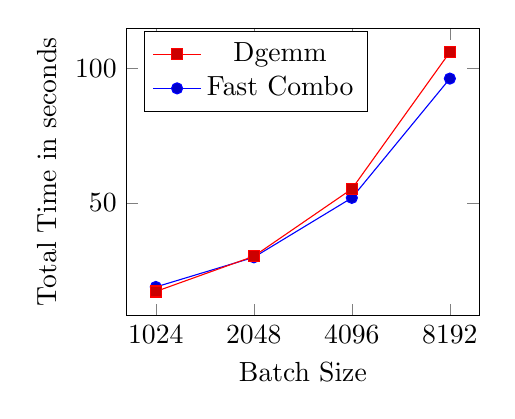
\begin{tikzpicture}
    \begin{axis}[
        width=.5\textwidth,
        xmode=log,
        log basis x={2},
        xlabel=Batch Size, 
        ylabel=Total Time in seconds,
        legend style={at={(.05,.85)},anchor=west},
        xtick={1024,2048,4096,8192},
        xticklabels={1024,2048,4096,8192},
            /pgf/number format/.cd, 1000 sep={},
            reverse legend,
    ]
    \addplot 
        coordinates {(8192,96.19704151153564) (4096,51.911903381347656)
             (2048,29.849395275115967) (1024,18.838172435760498)};
    \addplot 
        coordinates {(8192,106.00743579864502) (4096,55.22960305213928) 
            (2048,30.237940549850464) (1024,17.160202264785767)};
    \legend{Fast Combo,Dgemm}
    \end{axis}
\end{tikzpicture}
\caption{Total time test on VGG-11 with 6 threads}
\label{fig:vgg}
\end{figure}

\subsection{VGG-11 Network}
\RZ{description of the model of VGG-11 and VGG-19?}




% \subsection{Accuracy}

\subsection{Performance}
\RZ{VGG-11 fully connected layer: BS x 25K x 4K / BS x 4K x 4K / BS x 4K x 1K? with plot}
\cref{fig:vgg}
\RZ{Fast Combo: 525, 442, 242}


\section{Conclusion}

Arbitrary Precision Approximating algorithms offer significant practical performance improvements over exact fast matrix multiplication algorithms.
They outperform classical matrix multiplication at smaller matrix dimensions and yield greater benefits as matrix dimensions increase.
APA algorithms sacrifice accuracy, achieving error of only a fractional root of the working precision, but they can be practical for applications that do not demand high accuracy.
The results presented here show that neural network training, particularly for Multi-Layer Perceptron networks, is robust to such matrix multiplication error, and APA algorithms are a useful tool for accelerating the costly training computations.
We observe that for APA algorithms offering a theoretical speedup of up to 39\%, we can achieve up to 28\% and 21\% improvements for single- and multi-threaded implementations of individual matrix multiplications, respectively, which translate to up to 13\% speedup in overall training time on a multicore CPU.

While the accuracy and performance results are promising for MLP networks and the MNIST dataset, we believe that APA algorithms can also be effective in state-of-the-art networks and more difficult machine learning problems.
For example, the VGG-19 network for large-scale visual recognition \cite{SZ15} is based on a deep convolutional network and is bottlenecked by large fully connected layers, including a layer with dimensions $25088\times 4096$, where APA algorithms can offer significant performance improvement.

As illustrated by Benson and Ballard \cite{BB15}, the highest performing fast algorithms for rectangular matrix multiplications often have dimensions that match the aspect ratio of the problem.
We consider in this paper only square matrix multiplications, and we see that square (or nearly square) dimensions of $\dims{4,4,4}$ and $\dims{4,4,2}$ are fastest.
Algorithms with more skewed aspect ratios will likely perform better for problems with matching skewed matrix multiplication dimensions.
We note that an algorithm for dimensions $\dims{m,n,k}$ can be translated into an algorithm for $\dims{n,m,k}$ and any other reordering of the dimensions \cite{BB15}.
For very large matrices, it may also be beneficial to consider more than one recursive step of the same algorithm or a combination of two or three different algorithms across recursive steps (uniform, non-stationary algorithms \cite{BBDLS16}).

Finally, we would like to extend the code generation techniques to other hardware platforms, including GPUs.
Because GPUs can offer higher efficiency for matrix multiplications, we wish to demonstrate the potential of APA algorithms in that environment.
Techniques used to accelerate Strassen's algorithm on the GPU \cite{HYvdG20,LAES13} can be generalized to other fast algorithms as done in work for multicore CPUs \cite{BB15,HRMvdG17}.
We believe improved performance benefits can be achieved by APA algorithms on GPU architectures due to the relatively higher memory bandwidth.

%\paragraph*{Acknowledgments}
%
%This material is based upon work supported by the NSF Grant No. CCF1942892 and a Wake Forest University Undergraduate Research and Creative Activities (URECA) Research Fellowship.

\newpage
\balance
\bibliographystyle{ACM-Reference-Format}
\bibliography{refs}

\end{document}
